\section{ARA Design, Layout, and History}

        The chip enabling connection of the FPGA with the ATRI is called the FX2.
        This chip was installed on ATRI's used for stations A1-A5 between 2013 and 2018. 
        The USB connection between the FX2 and the ATRI degrades overtime preventing the SBC from communicating with the FPGA, rendering the station unable to take data. 
        Full deprecation can be delayed by forcing the USB connection into slow speed. 
        Our stations tend to operate for a few months on low speed before connection to the FX2 chip is lost completely.
        Table~\ref{tab:station_daqboards} summarizes the types of DAQ boards, when they were in use, and other notes.
        This is an abbreviation of a Wikipedia page I authored, \href{https://mediawiki.icecube.wisc.edu/ara/index.php/ARA_Station_Histories}{ARA Station Histories}, which summarizes topline updates and downtimes for each station since they were installed. 
        This is not to be confused with the \href{https://mediawiki.icecube.wisc.edu/ara/index.php/Known_Station_Problems}{Known Station Problems} page, which contains notes about active and ongoing notes for each station, a page typically consulted by those on monitoring shifts. 

\section{Operations Pipeline}

    \subsection{Data Transfer Pipeline}
  
        The runs of data that are saved by each station are collected by the radio processing (Radproc) computer which is housed in the IceCube Laboratory (ICL). 
        This data transfer and any other communications with the stations is conducted over fiber optic cable buried in the ice. 
        These fiber optic cables pass through a series of patch panels to reach their destination. 
        Starting at Radproc, information travels over intranet to a White Rabbit Switch\footnote{\url{https://www.white-rabbit.tech/wr-technology}}, a network switch used to enable time synchronization between connected devices. 
        %Ethernet leaves the White Rabbit Switch and is converted by a Small Form-factor Pluggable (SFP) into an optical signal that then enters a fiber optic patch panel in the ICL. 
        Outgoing fiber optic cables exit the ICL and run down the West Tower into the West Tower Junction Box, where the second patch panel is and leads immediately to a third patch panel located in the same box. 
        Cables leaving the third patch panel are laid over 1~km and end at Wind Turbine 3 where they meet their fourth patch panel. 
        Bundles of fiber optic cables are then run to stations A1, A2, and A3. 
        At this point, 2 fiber optic cables in each bundle are connected to A1, A2, and A3 while the last 2 cables at A1 are connected to a switch directing fiber optic signal to A4 and the last 2 cables at A2 being connected to a switch directing signal to A5. 
        I compiled the mapping of all fibers from the ICL to ARA stations and the IceCube Surface Array into a spreadsheet that is available in \href{https://aradocs.wipac.wisc.edu/DocDB/DocumentDatabase}{ARA DocDB\#\#\#\#}.\footnote{\comment{I need to upload this file to DocDB then I'll get the number.}}

        % \begin{figure}
        %   \centering
        %   \begin{subfigure}[t]{0.18\textwidth}
        %     \centering
        %     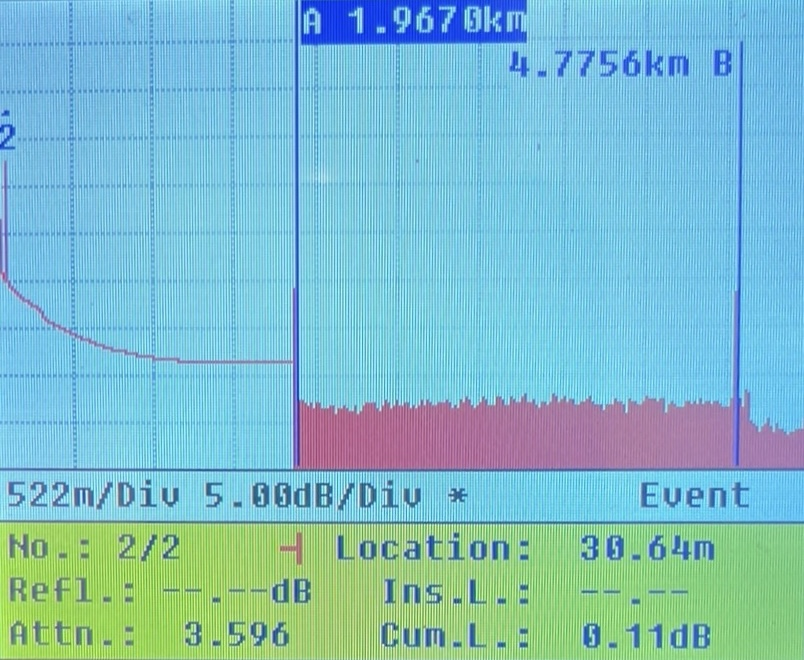
\includegraphics[
        %       width=\textwidth,
        %       alt={
        %         x
        %       }
        %       ]{sections/ARA/images/IMG_1742_FiberX_20250123_1445_toA3_fromICL_Abby.jpg} 
        %   \end{subfigure}
        %   ~
        %   \begin{subfigure}[t]{0.79\textwidth}
        %     \centering
        %     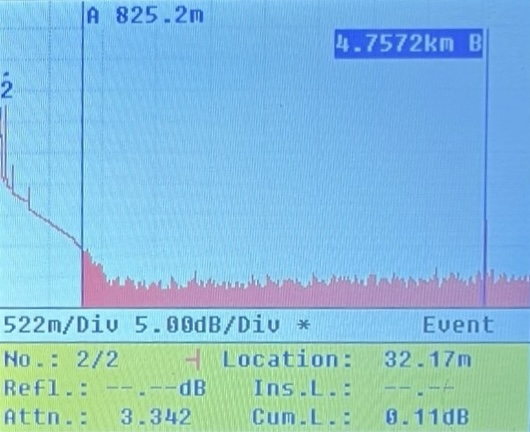
\includegraphics[
        %       width=\textwidth,
        %       alt={
        %         x
        %       }
        %       ]{sections/ARA/images/IMG_1744_FiberX_20250123_1452_toA3_fromICL_Abby.jpg}
        %   \end{subfigure}
        %   \caption{OTDR. Left, before cleaning. Right, after cleaning.}
        %   \label{fig:a3_otdr}
        % \end{figure}

        Note that, in January 2025, we discovered the fibers connecting the ICL patch panel port 19 and 20 to the West Tower Junction Box patch panel were reversed compared to previous documentation.
        This has been updated in the aforementioned DocDB article. 
        Handling of fibers in the West Tower Junction Box which connect the ICL to A3 via port 19 were handled unintentionally when installing the IceCube Surface Array extension. 
        Impurities may have been introduced into these fibers and the field team recommends retermination of the wires in the West Tower Junction Box in a future field season to restore network connection to A3.
        Since then, we have struggled to maintain network connection to A3. % and many Optical Time-Domain Reflectometer (OTDR) measurements have been conducted to calculate the distance to optical reflections caused by patch panels. 
        % On January 23, 2025 Delia Tosi and I ran OTDR measurements from the ICL to A3 and saw reflections consistent with Wind Turbine 3 around 2.0~km and at A3 around 4.8~km, but no reflections at the West Tower Junction Box at 300~m, shown on the left of Fig.~\ref{fig:a3_otdr}.
        % At this stage we did not have connection to A3 so we cleaned the fibers with electronics alcohol pads in the ICL and the West Tower Junction box then repeated the measurement where we saw reflections at the West Tower Junction Box and A3 but not at the closer Wind Turbine 3. 
        % After swapping out SFPs, fiber optics cables, and restarting the A3 power multiple times A3 came back online and took data for a few weeks before we lost connection again. 
        % OTDR measurements were repeated by IceCube Winterover Joe Baines-Holmeson March 7, 2025 where a steep power drop at 300~m was measured with no reflections. 
        % Oddly, some OTDR measurements still showed reflections at 4.7~km but still no reflections at 2~km at Wind Turbine 3. 
        % ^^^ I don't have this story nailed down well enough right now. I need to consult my notebook.

        % Would be nice to have a diagram of the networking

        ARA's power cabling follows a similar layout between the ICL and Wind Turbine 3. 
        Stations A1 and A4 are connected to the same power supply in the ICL, similar to the networking setup, however A2, A3, and A5 have their own power supplies\footnote{\comment{Are these separate power cables or does a power cable go into A1 and then a new cable connects A1 power to A4?}}. 
        A2 and A3 used to share a power supply but these stations drew too much power when being turned on after the power supplies experienced a full shut down, so they are now powered separately.

        The Radproc computer in the ICL collects all the data from A1-A5 and the Phased Array.
        $\sim \! 1\%$ of events in each run are randomly selected, forming our monitoring data sample. 
        The monitoring data is put into a data ``dropbox" (i.e. a directory titled \texttt{dropboxes}) going ``north'' and the full run file is put into a data drop box going ``south''. 
        These drop boxes are coordinated by IceCube data specialists. 
        The data in the ``north'' drop box is sent over satellite to the University of Wisconsin Madison (UW--Madison) for processing and used in monitoring and operations. 
        This data sample is automatically processed by an ARA Operations lead so collaborators may generate and monitor event displays and station metadata (temperature, event rates, etc) on \href{http://aware.wipac.wisc.edu}{AWARE}.
        The data in the ``south'' drop box is stored on hard drives (also referred to as ``tapes'') that are accumulated and shipped at the end of each calendar year. 
        These hard drives arrive at UW--Madison in the spring and are uploaded to the IceCube data warehouse in late spring and early summer.
  
    \subsection{Data Processing}
  
        Data straight from the hard drives are referred to as ``raw'' or ``L0'' data. 
        With some packages, like \texttt{pyaradisplay}\footnote{Documented in \href{https://aradocs.wipac.wisc.edu/cgi-bin/DocDB/ShowDocument?docid=937}{https://aradocs.wipac.wisc.edu/cgi-bin/DocDB/ShowDocument?docid=937} but updated in 2024 by John Kelley, Alan Salcedo Gomez, and me.}, one can plot waveforms however this does not include any calibrations and is not quickly readable for analysis.
        Therefore, once uploaded, A1-A5 L0 data is transformed into a ROOT~\citep{root} readable, L1 format by the ARA Mass Processing\footnote{
          \href{https://github.com/AndrewShultz/AraMassProcessing}{https://github.com/AndrewShultz/AraMassProcessing}, written by Andrew Schultz.
        } package and PA data is transformed by the NuPhase Rootification\footnote{
          \href{https://github.com/vPhase/nuphase_rootification}{https://github.com/vPhase/nuphase\_rootification}, written by me, based on scripts by Kaeli Hughes and the \href{https://github.com/vPhase/nuphaseroot}{\texttt{NuPhaseRoot}} and \href{https://github.com/vPhase/libnuphase}{\texttt{libNuPhase}} packages that were created by Cosmin Deaconu. 
          Note that the \texttt{NuPhase Rootification} package is in a private repository that cannot be viewed by those who are not members of the \href{https://github.com/vPhase}{\texttt{vPhase}} GitHub organization.
        } package.
        The process of transforming L0 into L1 data is called ``rootification'' or ``unpacking''\footnote{IceCube IT refers to the uploading of L0 data to the IceCube data warehouse as ``unpacking'' so I refer to the transformation of L0 into L1 data as ``rootification''. ARA collaborators may still use ``unpacking'' to describe L1 generation.}. 
        Colleagues at the University of Nebraska Lincoln rootify A1-A5 data under the supervision of Ilya Kravchenko while I have rootified PA data with advice from Cosmin Deaconu and Marco Muzio. 
        Over the past year I trained Sanyukta Agarwal at Kansas University to rootify PA data. 

        After ARA data has been rootified, the data is validated. 
        Some runs are too small and are logged as such in presentations on the ARA Analysis Call and pages like \href{https://mediawiki.icecube.wisc.edu/ara/index.php/2020_L0-L1_Unpacking_Notes}{the 2020 L0-L1 Unpacking Notes}. 
        A series of validation tests are performed to assess that the data has been unpacked properly and to identify any bad runs. 
        Some validation metrics include analyzing the number of samples in a waveform, sampling rate, waveform root mean square, and repeated event numbers.
        
        After data has been rootified, data is split into two samples: a full 100\% sample and a smaller 10\% sample\footnote{
            The smaller A1-A5 sample is technically reduced to a 9.5\% sample, but we round this to 10\% when referring to it.
        }. 
        Data analyses are typically built on the 10\% data sample then applied to the 100\% sample, as a blinding strategy. 
        For an experiment looking for rare data in a band of electromagnetic frequencies that strongly overlaps with anthropogenic backgrounds (e.g. snowmobile spark plugs, radios, airplanes, weather balloons, etc), building an analysis on only 10\% of the data has proven risky. 
        For example, unpredicted backgrounds have survived final event selection in some analyses and other analyses have removed an excessive number of events to avoid surviving backgrounds, both reducing analysis impact. 
        It would benefit us to consider other blinding strategies in addition to this one.

